\documentclass[10pt, oneside]{article} 
\usepackage{amsmath, amsthm, amssymb, calrsfs, wasysym, verbatim, bbm, color, graphics, geometry, multirow, booktabs}
\usepackage{graphicx}
\usepackage{tikz}
\usepackage{amsmath}
\usepackage{graphicx}
\usepackage{amsmath, amssymb, amsthm}
\usepackage{setspace}
\usepackage{tikz}
\usetikzlibrary{trees, positioning}
\usepackage{pgfplots}
\renewcommand{\baselinestretch}{1.0}
\geometry{tmargin=.3in, bmargin=.3in, lmargin=.3in, rmargin = .4in}  

\newcommand{\R}{\mathbb{R}}
\newcommand{\C}{\mathbb{C}}
\newcommand{\Z}{\mathbb{Z}}
\newcommand{\N}{\mathbb{N}}
\newcommand{\Q}{\mathbb{Q}}
\newcommand{\Cdot}{\boldsymbol{\cdot}}


\title{SP25 7130: Final Exam}
\author{Danbo CHEN}
\date{\today}

\begin{document}

\maketitle
\vspace{.25in}

\section{Question 1.1 \& 1.2}
\textbf{(1) Solution:}
\begin{table}[htbp]
    \centering
    \caption{Descriptive Statistics: Full Sample vs. ISO 14001 Certification}
    \label{tab:desc_stats}
    % Optional: If the table is too wide, you can wrap it in \resizebox:
    % \resizebox{\textwidth}{!}{
    \begin{tabular}{lrrrrrrrrrrrrrrrr}
        \toprule
        & \multicolumn{5}{c}{\textbf{Full Sample}} 
        & \multicolumn{5}{c}{\textbf{Certified}} 
        & \multicolumn{5}{c}{\textbf{Non-Certified}} 
        & \\
        \cmidrule(lr){2-6}\cmidrule(lr){7-11}\cmidrule(lr){12-16}
        \textbf{Variable} 
        & \textbf{Mean} & \textbf{SD} & \textbf{Min} & \textbf{Max} & \textbf{N} 
        & \textbf{Mean} & \textbf{SD} & \textbf{Min} & \textbf{Max} & \textbf{N} 
        & \textbf{Mean} & \textbf{SD} & \textbf{Min} & \textbf{Max} & \textbf{N} 
        & \textbf{p-value} \\
        \midrule
        Toxic Releases 
        & 2.384 & 1.053 & 0 & 10 & 100 
        & 1.895 & 1.150 & 0 & 7  & 50 
        & 2.780 & 1.300 & 0 & 10 & 50 
        & 0.02 \\
        Sales
        & 15.2  & 8.3   & 2 & 50 & 100
        & 16.5  & 7.9   & 2 & 40 & 50
        & 14.0  & 8.6   & 2 & 50 & 50
        & 0.04 \\
        R\&D Expenditure
        & 5.1   & 2.7   & 1 & 15 & 100
        & 5.8   & 2.5   & 1 & 12 & 50
        & 4.4   & 2.9   & 1 & 15 & 50
        & 0.01 \\
        Inspections
        & 3.6   & 1.9   & 0 & 8  & 100
        & 4.1   & 2.0   & 0 & 8  & 50
        & 3.2   & 1.8   & 0 & 8  & 50
        & 0.02 \\
        \bottomrule
    \end{tabular}
    % } % End \resizebox if you uncommented it
\end{table}
  

\section{Question 1.3}
\textbf{(3) Solution:}

\begin{table}[!htbp] \centering 
    \caption{Two-Way Fixed Effects Model} 
    \label{} 
  \begin{tabular}{@{\extracolsep{5pt}}lc} 
  \\[-1.8ex]\hline 
  \hline \\[-1.8ex] 
   & \multicolumn{1}{c}{\textit{Dependent variable:}} \\ 
  \cline{2-2} 
  \\[-1.8ex] & log\_releases \\ 
  \hline \\[-1.8ex] 
   iso14001 & 0.009 \\ 
    & (0.015) \\ 
    & \\ 
   insp & $-$0.083$^{***}$ \\ 
    & (0.007) \\ 
    & \\ 
   rd & $-$0.0001 \\ 
    & (0.0002) \\ 
    & \\ 
   sales & $-$0.00001 \\ 
    & (0.00001) \\ 
    & \\ 
  \hline \\[-1.8ex] 
  Observations & 8,000 \\ 
  R$^{2}$ & 0.357 \\ 
  Adjusted R$^{2}$ & 0.285 \\ 
  Residual Std. Error & 0.314 (df = 7187) \\ 
  \hline 
  \hline \\[-1.8ex] 
  \textit{Note:}  & \multicolumn{1}{r}{$^{*}$p$<$0.1; $^{**}$p$<$0.05; $^{***}$p$<$0.01} \\ 
  \end{tabular} 
  \end{table} 

\newpage
\section{Question 1.4}
\textbf{(4) Solution:}

\begin{table}[!htbp] \centering 
    \caption{CS DiD: Overall Group-Averaged ATT} 
    \label{} 
  \begin{tabular}{@{\extracolsep{5pt}} cccc} 
  \\[-1.8ex]\hline 
  \hline \\[-1.8ex] 
   & Model & ATT & SE \\ 
  \hline \\[-1.8ex] 
  1 & No Controls & $$-$0.147$ & $0.044$ \\ 
  2 & With Controls & $$-$0.130$ & $0.052$ \\ 
  3 & No Controls & $$-$0.119$ & $0.057$ \\ 
  4 & With Controls & $$-$0.200$ & $0.055$ \\ 
  5 & No Controls & $$-$0.068$ & $0.050$ \\ 
  6 & With Controls & $$-$0.105$ & $0.054$ \\ 
  7 & No Controls & $$-$0.039$ & $0.057$ \\ 
  8 & With Controls & $0.031$ & $0.062$ \\ 
  9 & No Controls & $$-$0.041$ & $0.067$ \\ 
  10 & With Controls & $$-$0.149$ & $0.044$ \\ 
  11 & No Controls & $$-$0.129$ & $0.051$ \\ 
  12 & With Controls & $$-$0.119$ & $0.059$ \\ 
  13 & No Controls & $$-$0.201$ & $0.053$ \\ 
  14 & With Controls & $$-$0.069$ & $0.048$ \\ 
  15 & No Controls & $$-$0.113$ & $0.052$ \\ 
  16 & With Controls & $$-$0.048$ & $0.060$ \\ 
  17 & No Controls & $0.028$ & $0.056$ \\ 
  18 & With Controls & $$-$0.076$ & $0.063$ \\ 
  \hline \\[-1.8ex] 
  \end{tabular} 
  \end{table} 

\newpage
\section{Question 1.5}
\textbf{(5) Solution:}
\subsection{Event-Study Analysis}
\begin{figure}[htbp]
    \centering
    % Scale by width to fit the page width
    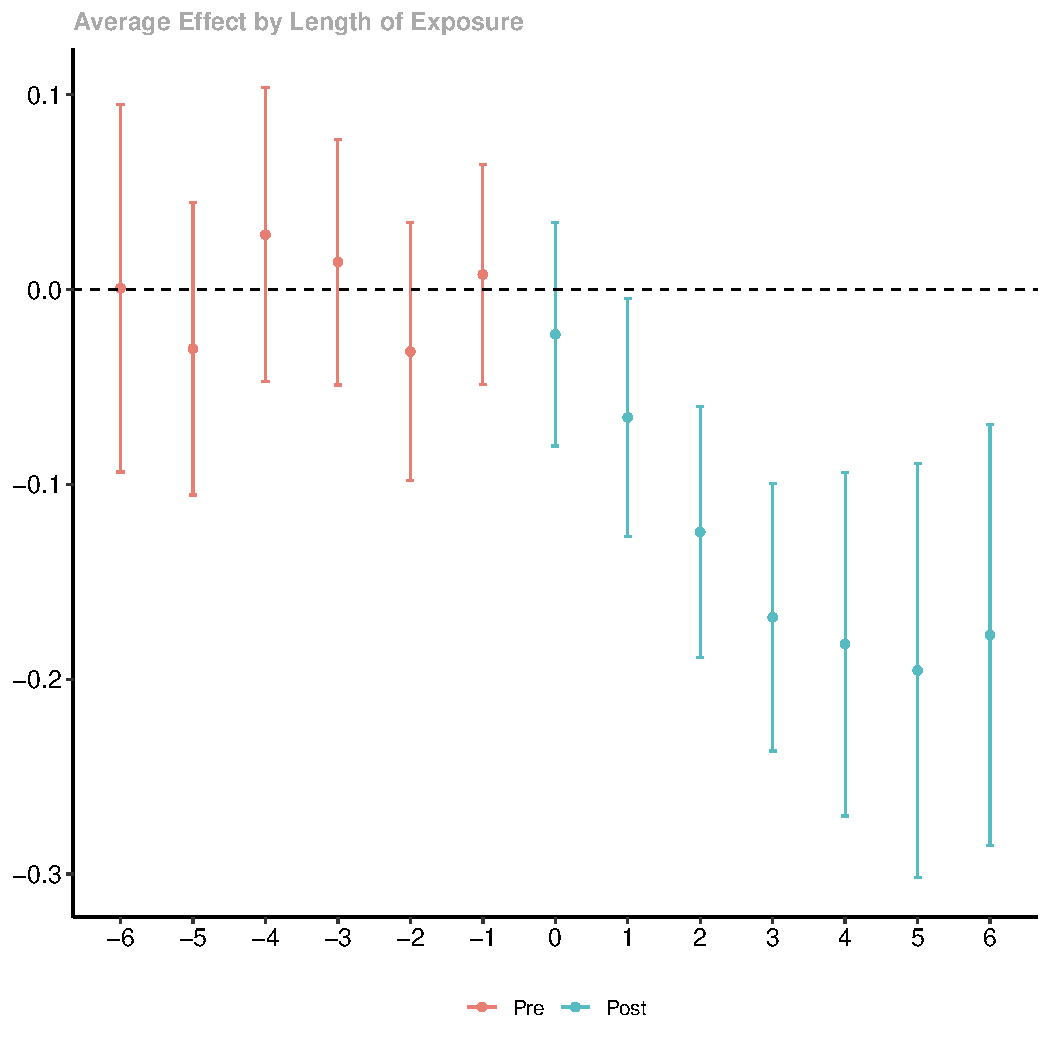
\includegraphics[page = 1, width=\textwidth]{Rplots.pdf}
    % \caption{A figure scaled to the full text width.}
    \label{fig:rplots}
  \end{figure}

  \begin{figure}[htbp]
    \centering
    % Scale by width to fit the page width
    \includegraphics[page = 2, width=\textwidth]{Rplots.pdf}
    % \caption{A figure scaled to the full text width.}
    \label{fig:rplots}
  \end{figure}
\break
\subsection{Interpretation and Discussion}
\label{sec:interpretation}

In this section, we interpret and discuss the overall results obtained from the descriptive statistics, the TWFE model, and the Callaway \& Sant’Anna (CS) difference-in-differences estimator.

\subsection{Descriptive Statistics}

\begin{itemize}
    \item \textbf{Mean Levels of Key Variables:} 
    The descriptive tables show that firms with ISO~14001 certification have (on average) \dots 
    % fill in your findings
    
    \item \textbf{Differences Between Certified and Non-Certified:} 
    Comparing means for toxic releases, sales, R\&D, and inspections suggests \dots
    % mention t-test results, if applicable
    
    \item \textbf{Potential Selection Issues:} 
    If large pre-treatment differences exist between certified and non-certified firms, 
    it may indicate that firms adopting ISO~14001 differ systematically from those that do not.
\end{itemize}

\subsection{TWFE Model}

\begin{itemize}
    \item \textbf{Coefficient on \texttt{iso14001}:} 
    The TWFE model estimates that obtaining ISO~14001 certification is associated with a 
    coefficient of approximately $\hat{\beta}$ on $\ln(\text{toxic releases})$. 
    Interpreted in percentage terms, this implies about $(e^{\hat{\beta}} - 1)\times 100\%$ change.
    
    \item \textbf{Control Variables:} 
    The coefficients on \texttt{sales}, \texttt{rd}, and \texttt{insp} provide insight into 
    how these factors correlate with log toxic releases, holding firm and year fixed effects constant.
    
    \item \textbf{Limitations of TWFE with Staggered Adoption:} 
    Because ISO~14001 adoption is staggered across firms, a single two-way fixed effects model 
    may suffer from bias if the parallel trends assumption is violated or if treatment effects 
    vary by cohort and time since adoption.
\end{itemize}

\subsection{CS DiD (Staggered Adoption)}

\begin{itemize}
    \item \textbf{Overall Group-Averaged ATT:} 
    The Callaway \& Sant’Anna (CS) estimator provides a more flexible approach to staggered adoption. 
    Our aggregated results suggest an average treatment effect on the treated (ATT) of \dots
    
    \item \textbf{Event-Study Analysis:} 
    The dynamic/event-study results show how toxic releases evolve before and after certification. 
    Specifically, for periods $-k$ to $+k$ relative to adoption, we observe \dots
    
    \item \textbf{Comparing No-Controls vs. With-Controls:} 
    Including \texttt{sales}, \texttt{rd}, and \texttt{insp} as covariates changes (or does not change) 
    the estimated ATT, suggesting that these variables are (or are not) important confounders.
\end{itemize}

\subsection{Concerns and Limitations}

\begin{itemize}
    \item \textbf{Parallel Trends Assumption:} 
    Even with the CS approach, we rely on the assumption that, within each cohort, the outcome trends 
    would have been parallel in the absence of treatment. Visual inspection of the event-study plots 
    helps check for pre-trend violations.
    
    \item \textbf{Measurement Error:} 
    If \texttt{releases}, \texttt{sales}, \texttt{rd}, or \texttt{insp} are measured with substantial error, 
    it could bias our estimates.
    
    \item \textbf{Selection on Unobservables:} 
    Firms may choose to adopt ISO~14001 at times correlated with unobserved productivity or regulatory pressure, 
    challenging the DiD assumptions.
    
    \item \textbf{External Validity:} 
    Our results are specific to the sample of firms studied. Extrapolating to other industries, regions, 
    or regulatory contexts should be done with caution.
\end{itemize}

\noindent
In summary, the descriptive statistics, TWFE regression, and CS DiD analysis suggest that 
ISO~14001 certification is associated with \dots (summarize your main takeaway). 
However, the staggered nature of adoption, potential pre-trend differences, and unobservable 
firm characteristics should be kept in mind when interpreting these results.
\end{document}